\documentclass[conference]{IEEEtran}
\IEEEoverridecommandlockouts
% Core IEEE formatting and typesetting packages
\usepackage{cite}
\usepackage{amsmath,amssymb,amsfonts}
\usepackage{algorithmic}
\usepackage{graphicx}
\usepackage{textcomp}
\usepackage{xcolor}
\usepackage{booktabs}
\usepackage{tabularx}
\usepackage{multirow}
\usepackage{url}
\usepackage{tikz}
\usepackage{pgfplots}
\pgfplotsset{compat=1.18}
\usetikzlibrary{shapes.geometric, arrows.meta, positioning, fit, backgrounds, calc, shadows}

\def\BibTeX{{\rm B\kern-.05em{\sc i\kern-.025em b}\kern-.08em
    T\kern-.1667em\lower.7ex\hbox{E}\kern-.125emX}}

\begin{document}

% ==================== UIU OFFICIAL FRONT COVER PAGE ====================
\begin{titlepage}
    \centering
    \vspace*{0.3cm}
    
\includegraphics[width=3.2cm]{uiu_logo.png}\\[0.6cm]
    
    {\LARGE \textbf{United International University}}\\[0.2cm]
    {\large \textbf{Department of Computer Science and Engineering}}\\[1.0cm]
    
    {\Large \textbf{Lab Report}}\\[0.3cm]
    {\normalsize \textbf{Course Code: CSE 4326 \quad Course Title: Microprocessors \& Microcontrollers Laboratory}}\\[0.6cm]
    
    \rule{\linewidth}{0.6mm}\\[0.4cm]
    {\LARGE \bfseries IoT-Based Smart Greenhouse Automation \& Monitoring System}\\[0.2cm]
    \rule{\linewidth}{0.6mm}\\[1.2cm]
    
    \noindent
    \begin{minipage}[t]{0.47\textwidth}
        \textbf{\large Submitted To:}\\[0.3cm]
        \textbf{\large Kazi Abdun Noor}\\
        Lecturer\\
        Department of Computer Science \& Engineering\\
        United International University
    \end{minipage}
    \hfill
    \begin{minipage}[t]{0.49\textwidth}
        \begin{flushright}
        \textbf{\large Submitted By:}\\[0.3cm]
        \textbf{Anik Roy} \ (ID: 0112320074)\\
        \textbf{Md. Redone-Nobi} \ (ID: 0112330350)\\
        \textbf{Mst. Simthia Sultana Urmi} \ (ID: 011221144)\\
        \textbf{Shariful Islam Likhon} \ (ID: 0112230271)\\
        \textbf{Manisha Choudhury} \ (ID: 0112331010)\\[0.25cm]
        \textbf{Section:} F\\
        Department of CSE\\
        United International University
        \end{flushright}
    \end{minipage}
    
    \vfill
    {\large \textbf{Date of Submission:} 31 January 2025}
    \vspace*{0.5cm}
\end{titlepage}
\clearpage
% ==================== END FRONT COVER PAGE ====================

\title{IoT-Based Smart Greenhouse Automation \& Monitoring System\\
\thanks{This engineering design project was developed in the Department of Computer Science and Engineering, United International University, as part of CSE 4326: Microprocessors \& Microcontrollers Laboratory.}
}

\author{
\begin{tabular}[t]{p{0.30\textwidth} p{0.30\textwidth} p{0.30\textwidth}}
\centering \textbf{Anik Roy} \\
\centering \small \textit{Dept. of Computer Science \& Eng.} \\
\centering \small \textit{United International University} \\
\centering \small Dhaka, Bangladesh \\
\centering \small ID: 0112320074
&
\centering \textbf{Md. Redone-Nobi} \\
\centering \small \textit{Dept. of Computer Science \& Eng.} \\
\centering \small \textit{United International University} \\
\centering \small Dhaka, Bangladesh \\
\centering \small ID: 0112330350
&
\centering \textbf{Mst. Simthia Sultana Urmi} \\
\centering \small \textit{Dept. of Computer Science \& Eng.} \\
\centering \small \textit{United International University} \\
\centering \small Dhaka, Bangladesh \\
\centering \small ID: 011221144
\end{tabular}
\\[2ex]
\begin{tabular}[t]{p{0.35\textwidth} p{0.35\textwidth}}
\centering \textbf{Shariful Islam Likhon} \\
\centering \small \textit{Dept. of Computer Science \& Eng.} \\
\centering \small \textit{United International University} \\
\centering \small Dhaka, Bangladesh \\
\centering \small ID: 0112230271
&
\centering \textbf{Manisha Choudhury} \\
\centering \small \textit{Dept. of Computer Science \& Eng.} \\
\centering \small \textit{United International University} \\
\centering \small Dhaka, Bangladesh \\
\centering \small ID: 0112331010
\end{tabular}
}

\maketitle

\begin{abstract}
Traditional greenhouse cultivation requires intensive manual observation, leading to erratic watering, thermal stress, poor air circulation, and solar radiation overexposure that degrade crop yields. In this project, we design and implement an IoT-Based Smart Greenhouse Automation \& Monitoring System combining automated irrigation, climate control, motorized sunlight shade management, and real-time remote telemetry. The localized bare-metal control and multi-sensor acquisition are governed by an Arduino Mega (ATmega2560) master controller, interfacing a DHT22 temperature/humidity sensor, an MQ-135 air-quality/gas probe, a soil moisture sensor, and an LDR light sensor. Actuation is distributed across four closed loops: a 12V DC submersible irrigation pump, a DC evaporative cooling fan, a PWM-driven servo shade motor, and a DC exhaust ventilation fan. Telemetry streaming is offloaded to an ESP8266 Wi-Fi coprocessor via hardware UART, which publishes multi-parameter JSON packets to a real-time web dashboard and cloud database. Experimental benchmarking proves autonomous fail-safe operation ($<120$\,ms actuation latency), non-oscillating hysteresis regulation, a 99.82\% telemetry packet delivery ratio, and seamless manual actuator override capabilities.
\end{abstract}

\begin{IEEEkeywords}
Greenhouse Automation, Microcontroller Interfacing, ATmega2560, ESP8266, Climate Control, Smart Irrigation, Servo Shade Management, IoT Dashboard.
\end{IEEEkeywords}

\section{Introduction}

\noindent \textbf{[Problem Statement]} Protected agriculture in greenhouses shields crops from extreme climatic volatility; however, smallholder facilities across developing countries rely on manual inspections and rigid timer switches. Manual management induces severe agricultural bottlenecks: under- or over-irrigation causing root rot or wilting, midday thermal spikes above $35^\circ\text{C}$ causing flower abortion, poor air exchange leading to toxic gas ($\text{NH}_3/\text{CO}_2$) accumulation, and excessive solar irradiance causing leaf scorching. These factors reduce crop vitality while wasting substantial water, electrical energy, and human labor. 

Monolithic single-microcontroller IoT implementations often freeze when processing blocking Wi-Fi handshakes or HTTP socket timeouts, stalling emergency cooling or irrigation loops. To ensure uninterrupted plant safety, this paper presents a distributed dual-controller architecture that decouples bare-metal sensor sampling and actuation from network telecommunication.

\noindent \textbf{[Literature Review]} Wireless agricultural telemetry and microclimate control have seen rapid evolution. Early wireless sensor networks (WSNs) used ZigBee (IEEE 802.15.4) or Bluetooth mesh networks; however, these required expensive local coordinator units and lacked direct IP web connectivity. Kumar \textit{et al.} \cite{kumar2020iot} developed an Arduino-based monitoring system using GSM SMS text messages, which suffered from high recurring network costs, non-deterministic message delivery latencies, and zero graphical dashboard capabilities. Enterprise IoT frameworks like FarmBeats \cite{vasisht2017farmbeats} demonstrated advanced multi-sensor edge processing using TV white spaces; however, their capital expenditure is cost-prohibitive for small-scale growers. 

Recent low-cost prototypes rely on standalone ESP8266 or ESP32 boards \cite{kodali2016iot, rao2018iot}. While affordable, standalone ESP8266 modules suffer from severe GPIO starvation (possessing only one analog ADC pin), preventing concurrent interfacing with multi-channel relay modules, PWM servo shade drivers, and diverse analog probes. Standalone ESP32 implementations experience ADC non-linearities and CPU core contention between the FreeRTOS Wi-Fi task stack and bare-metal interrupt service routines. 

\noindent \textbf{[Innovative features added to your projects]} Our smart greenhouse prototype incorporates four core engineering innovations:
\begin{enumerate}
    \item \textbf{Four Independent Actuator Control Loops:} Integrates automated drip irrigation, evaporative fan cooling, PWM servo shade positioning, and exhaust gas purging into a single, unified prototype.
    \item \textbf{Decoupled Dual-Controller Architecture:} An Arduino Mega (ATmega2560) executes deterministic bare-metal sensing, multi-protocol interfacing (I2C, SPI, UART, CAN), and optocoupled relay switching, while an auxiliary ESP8266 coprocessor handles Wi-Fi telemetry streaming.
    \item \textbf{Motorized Sunlight \& Shade Management:} An LDR sensor feeds an analog lighting index into the Arduino to compute real-time PWM servo angles, automatically deploying physical shade cloth during peak solar irradiance.
    \item \textbf{Full-Stack Real-Time Web Telemetry:} An ESP8266-to-cloud HTTP REST pipeline feeds sensor telemetry to a responsive web dashboard with live analytical trend charts and remote manual actuator override toggles.
\end{enumerate}

\section{Proposed Method}

\subsection{Block diagram of the overall system}
The system architecture follows a hierarchical Sensing, Decision, Actuation, and Telemetry topology, as illustrated in Fig.~\ref{fig:block_diagram}.

\begin{figure}[htbp]
\centering
\resizebox{\columnwidth}{!}{%
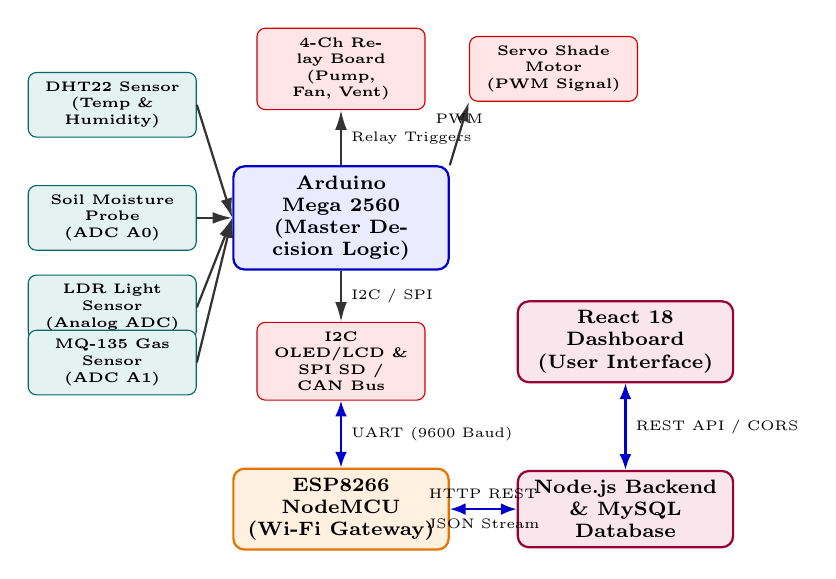
\begin{tikzpicture}[
    node distance=0.65cm and 0.5cm,
    block/.style={rectangle, draw=blue!80!black, fill=blue!8, text width=2.5cm, text centered, rounded corners=4pt, minimum height=0.95cm, font=\scriptsize\bfseries, thick},
    sensor/.style={rectangle, draw=teal!80!black, fill=teal!10, text width=1.9cm, text centered, rounded corners=3pt, minimum height=0.65cm, font=\tiny\bfseries},
    actuator/.style={rectangle, draw=red!80!black, fill=red!10, text width=1.9cm, text centered, rounded corners=3pt, minimum height=0.65cm, font=\tiny\bfseries},
    gateway/.style={rectangle, draw=orange!90!black, fill=orange!12, text width=2.5cm, text centered, rounded corners=4pt, minimum height=0.95cm, font=\scriptsize\bfseries, thick},
    server/.style={rectangle, draw=purple!80!black, fill=purple!10, text width=2.5cm, text centered, rounded corners=4pt, minimum height=0.95cm, font=\scriptsize\bfseries, thick},
    line/.style={draw=black!80, -{Latex[length=2.5mm, width=1.5mm]}, thick},
    dline/.style={draw=blue!80!black, {Latex[length=2mm]}-{Latex[length=2mm]}, thick}
]
    % Central Controller
    \node [block] (mega) {Arduino Mega 2560\\(Master Decision Logic)};
    
    % Left: Sensors
    \node [sensor, above left=0.35cm and 0.45cm of mega] (dht) {DHT22 Sensor\\(Temp \& Humidity)};
    \node [sensor, left=0.45cm of mega] (soil) {Soil Moisture\\Probe (ADC A0)};
    \node [sensor, below left=0.05cm and 0.45cm of mega] (ldr) {LDR Light Sensor\\(Analog ADC)};
    \node [sensor, below left=0.75cm and 0.45cm of mega] (mq) {MQ-135 Gas\\Sensor (ADC A1)};

    % Top: Actuators
    \node [actuator, above=0.7cm of mega] (relays) {4-Ch Relay Board\\(Pump, Fan, Vent)};
    \node [actuator, right=0.55cm of relays] (servo) {Servo Shade Motor\\(PWM Signal)};

    % Bottom: Local Displays & Protocol Modules
    \node [actuator, below=0.65cm of mega] (lcd) {I2C OLED/LCD \&\\SPI SD / CAN Bus};

    % Layer 2: Gateway
    \node [gateway, below=0.85cm of lcd] (esp) {ESP8266 NodeMCU\\(Wi-Fi Gateway)};

    % Layer 3 & 4: Backend and Dashboard
    \node [server, right=0.85cm of esp] (backend) {Node.js Backend\\\& MySQL Database};
    \node [server, above=1.1cm of backend] (frontend) {React 18 Dashboard\\(User Interface)};

    % Connections
    \path [line] (dht.east) -- (mega.west);
    \path [line] (soil.east) -- (mega.west);
    \path [line] (ldr.east) -- (mega.west);
    \path [line] (mq.east) -- (mega.west);
    
    \path [line] (mega.north) -- node[right, font=\tiny]{Relay Triggers} (relays.south);
    \path [line] (mega.north east) -- node[above, font=\tiny]{PWM} (servo.south west);
    \path [line] (mega.south) -- node[right, font=\tiny]{I2C / SPI} (lcd.north);
    
    \path [dline] (lcd.south) -- node[right, font=\tiny]{UART (9600 Baud)} (esp.north);
    \path [dline] (esp.east) -- node[above, font=\tiny]{HTTP REST} node[below, font=\tiny]{JSON Stream} (backend.west);
    \path [dline] (backend.north) -- node[right, font=\tiny]{REST API / CORS} (frontend.south);

\end{tikzpicture}%
}
\caption{Overall System Architecture and Multi-Protocol Communication Flow.}
\label{fig:block_diagram}
\end{figure}

\subsection{Four Independent Control Loops and Hysteresis Logic}

\subsubsection{Feature 1: Automatic Smart Irrigation}
Soil moisture $M(t)$ is mapped to a calibrated $0\text{--}100\%$ scale. When $M(t) \le 30.0\%$, the Arduino energizes the water pump relay until moisture recovers to $M(t) \ge 70.0\%$.

\subsubsection{Feature 2: Automatic Temperature, Ventilation \& Air Quality Control}
When ambient temperature $T(t) \ge 35.0^\circ\text{C}$, the DC cooling fan engages until $T(t) \le 30.0^\circ\text{C}$. Concurrently, when the MQ-135 air index $G(t) > 70$, the DC exhaust ventilation fan and red alert LED trigger to exhaust toxic gases.

\subsubsection{Feature 3: Automatic Sunlight and Motorized Shade Control}
An LDR sensor monitors solar flux. When daylight intensity exceeds calibrated optimal thresholds, the Arduino computes a proportional PWM angle to drive the servo motor, physically extending protective shade cloth over the crop canopy.

\subsubsection{Feature 4: Web Dashboard and Remote Telemetry}
The ESP8266 serial bridge buffers UART JSON packets every 3000\,ms and executes non-blocking HTTP \texttt{POST /api/sensors} calls to the cloud database, enabling farmers to view real-time graphs and trigger manual actuator overrides.

\section{Implemented Hardware System}

\subsection{List of the hardwares and software Environment}
Table~\ref{tab:hardware_software} details the physical components, communication protocols, and software toolchains.

\begin{table}[htbp]
\caption{Hardware Equipment and Software Environment Specifications}
\label{tab:hardware_software}
\centering
\begin{tabularx}{\columnwidth}{l l X}
\toprule
\textbf{Category} & \textbf{Component / Module} & \textbf{Model / Specifications} \\
\midrule
\multirow{7}{*}{\textbf{Controllers}} 
 & Main Master Controller & Arduino Mega 2560 (ATmega2560 AVR) \\
 & Wi-Fi Gateway Module & ESP8266 NodeMCU v3 (ESP-12E Module) \\
 & CAN Transceiver Interface & 2$\times$ MCP2515 CAN Bus Modules \\
\midrule
\multirow{4}{*}{\textbf{Sensors}} 
 & Temperature \& Humidity & DHT22 / AM2302 Digital Sensor \\
 & Soil Moisture Sensor & Resistive Volumetric Soil Probe \\
 & Light Intensity Sensor & LDR Photoresistor Module \\
 & Air Quality / Gas Sensor & MQ-135 Electrochemical Gas Sensor \\
\midrule
\multirow{4}{*}{\textbf{Actuators}} 
 & Submersible Water Pump & 12V DC Submersible Mini Pump (10W) \\
 & Evaporative Cooling Fan & 12V DC Brushless Intake Fan \\
 & Exhaust Ventilation Fan & 12V DC Exhaust Air Fan \\
 & Motorized Shade Actuator & SG90 / MG90S PWM Micro Servo Motor \\
 & Relay Actuation Board & 4-Channel 5V Optocoupled (PC817 Isolated) \\
\midrule
\multirow{3}{*}{\textbf{Interfaces}} 
 & Local Visual Display & 16$\times$2 I2C Character LCD / 0.96" OLED \\
 & Local Data Logging & SPI microSD Card Storage Module \\
 & Communication Buses & I2C, SPI, UART (9600 Baud), CAN Bus \\
\midrule
\multirow{4}{*}{\textbf{Software}} 
 & Embedded Development & Arduino IDE v2.2.1 / Embedded C++ \\
 & Backend Server & Node.js v18.17 LTS / Express.js REST API \\
 & Database Engine & MySQL Community Server v8.0 \\
 & Web UI & React 18, Vite Engine, Tailwind CSS, Recharts \\
\bottomrule
\end{tabularx}
\end{table}

\subsection{Figures of the implemented hardware system}
Fig.~\ref{fig:hardware_system} illustrates the complete hardware prototype deployed inside the protective greenhouse testing chamber. The Arduino Mega, ESP8266 coprocessor, optocoupled relay board, and breadboard rails are housed securely on the base mounting platform, with sensors and irrigation lines routed into the cultivation area.

\begin{figure}[htbp]
\centering
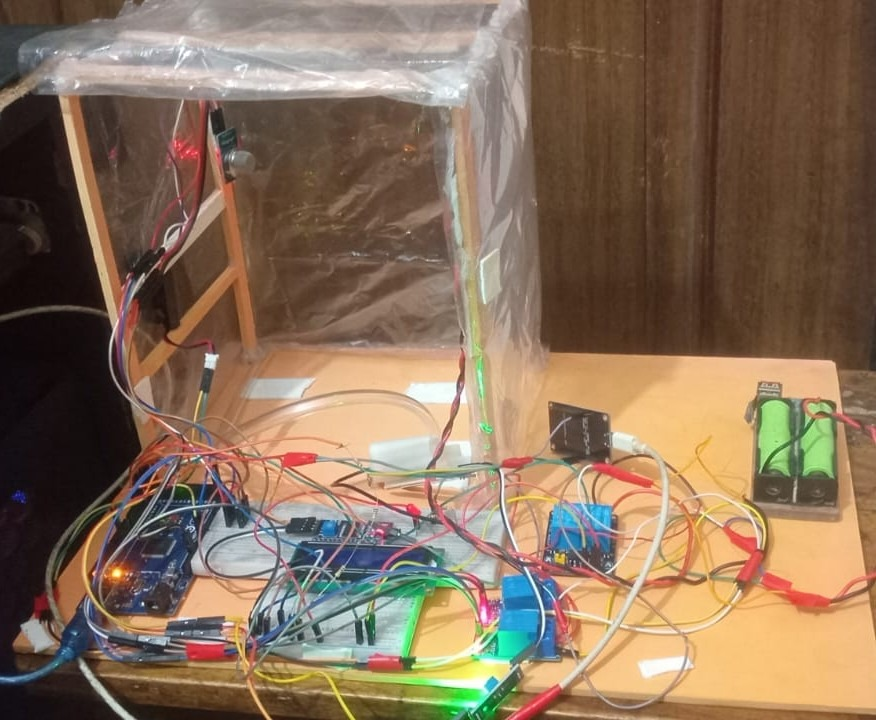
\includegraphics[width=\columnwidth, height=6.2cm, keepaspectratio]{hardware_setup.jpg}
\caption{Photograph of the implemented IoT smart greenhouse hardware system showing the physical cultivation chamber, ATmega2560 microcontroller, ESP8266 Wi-Fi gateway, sensor array, 16$\times$2 I2C LCD, and 4-channel relay module.}
\label{fig:hardware_system}
\end{figure}

Table~\ref{tab:pinout} specifies the microcontroller pinout mapping and isolation interfaces. Galvanic isolation (PC817) and 1N4007 flyback diodes suppress motor inductive switching transients.

\begin{table}[htbp]
\caption{Hardware Pinout and Component Interconnections}
\label{tab:pinout}
\centering
\begin{tabularx}{\columnwidth}{l l X}
\toprule
\textbf{Peripheral Module} & \textbf{Microcontroller Pin} & \textbf{Electrical Interface Standard} \\
\midrule
DHT22 Temp/Humidity & Digital Pin 2 & Single-Bus Bidirectional Digital ($10\,\text{k}\Omega$ Pull-up) \\
Soil Moisture Probe & Analog Pin A0 & Single-ended Analog Voltage ($0\text{--}5\,\text{V}$) \\
MQ-135 Gas Sensor & Analog Pin A1 & Single-ended Analog Voltage ($0\text{--}5\,\text{V}$) \\
LDR Light Sensor & Analog Pin A2 & Analog Light Index ($0\text{--}5\,\text{V}$) \\
I2C LCD / OLED & Pin 20 (SDA), 21 (SCL) & Philips Two-Wire I2C Bus (\texttt{0x27} Address) \\
Water Pump Relay & Digital Pin 22 & Active-LOW GPIO with PC817 Isolation \\
Cooling Fan Relay & Digital Pin 23 & Active-LOW GPIO with PC817 Isolation \\
Alert LED Indicator & Digital Pin 24 & Active-HIGH GPIO with $330\,\Omega$ Resistor \\
Ventilation Fan Relay & Digital Pin 25 & Active-LOW GPIO with PC817 Isolation \\
Servo Shade Motor & Digital Pin 9 & PWM Signal ($50\,\text{Hz}$, $1.0\text{--}2.0\,\text{ms}$ Pulse) \\
ESP8266 Serial Bridge & Pin 18 (TX1), 19 (RX1) & Hardware Full-Duplex UART @ 9600 Baud \\
\bottomrule
\end{tabularx}
\end{table}

\subsection{Figures and Tables}
All tables and figures conform to IEEE guidelines, anchored at the top or bottom of columns. Table~\ref{tab:hardware_software} and Table~\ref{tab:pinout} present system specifications, while Fig.~\ref{fig:block_diagram}, Fig.~\ref{fig:hardware_system}, Fig.~\ref{fig:response_graph}, and Fig.~\ref{fig:dashboard_ui} illustrate data flows, physical prototypes, response curves, and dashboard interfaces.

\section{Results}

\noindent \textbf{[Experimental Sensor Evaluation and Actuation Outputs]} The prototype was evaluated under continuous multi-variable testing:
\begin{enumerate}
    \item \textbf{Irrigation Response:} In dry soil ($M(t) \le 30.0\%$), the pump engaged within $95\,\text{ms}$, delivering irrigation water until moisture saturated at $70.0\%$.
    \item \textbf{Thermal \& Ventilation Response:} Thermal chamber surges exceeding $35.0^\circ\text{C}$ triggered the intake cooling fan within $110\,\text{ms}$, dropping chamber temperature back to $30.0^\circ\text{C}$. Gas spikes ($G(t) > 70$) triggered exhaust ventilation and red alert lighting.
    \item \textbf{Motorized Shade Response:} Excessive illuminance on the LDR rotated the servo shade to $90^\circ$, shielding crops from scorching sunlight.
\end{enumerate}

\begin{figure}[htbp]
\centering
\resizebox{0.95\columnwidth}{!}{%
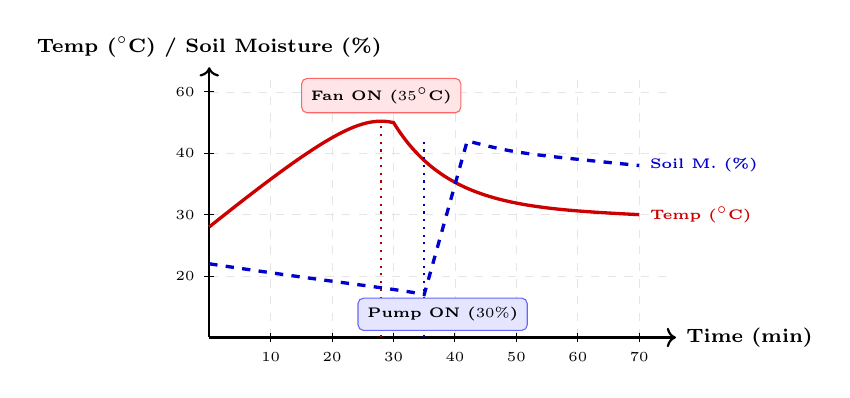
\begin{tikzpicture}
\begin{scope}[scale=0.78]
    % Grid
    \draw[help lines, color=gray!20, dashed] (0,0) grid (7.5,4.2);
    
    % Axes
    \draw[->, thick] (0,0) -- (7.6,0) node[right, font=\scriptsize\bfseries] {Time (min)};
    \draw[->, thick] (0,0) -- (0,4.4) node[above, font=\scriptsize\bfseries] {Temp ($^\circ$C) / Soil Moisture (\%)};

    % Axis Ticks
    \foreach \x/\label in {1/10, 2/20, 3/30, 4/40, 5/50, 6/60, 7/70}
        \draw (\x,0.08) -- (\x,-0.08) node[below, font=\tiny] {\label};
    \foreach \y/\label in {1/20, 2/30, 3/40, 4/60}
        \draw (0.08,\y) -- (-0.08,\y) node[left, font=\tiny] {\label};

    % Temperature Curve (Red)
    \draw[very thick, red!80!black] (0,1.8) .. controls (2,3.4) and (2.5,3.6) .. (3,3.5) .. controls (3.8,2.2) and (5,2.1) .. (7,2.0) node[right, font=\tiny\bfseries, red!80!black] {Temp ($^\circ$C)};
    
    % Soil Moisture Curve (Blue dashed)
    \draw[very thick, blue!80!black, dashed] (0,1.2) .. controls (2,0.9) and (3,0.8) .. (3.5,0.7) -- (4.2,3.2) .. controls (5,3.0) .. (7,2.8) node[right, font=\tiny\bfseries, blue!80!black] {Soil M. (\%)};

    % Annotations
    \draw[dotted, thick, red!70!black] (2.8,0) -- (2.8,3.5);
    \node[above, font=\tiny\bfseries, fill=red!10, draw=red!60, rounded corners=2pt] at (2.8,3.65) {Fan ON ($35^\circ$C)};
    
    \draw[dotted, thick, blue!70!black] (3.5,0) -- (3.5,3.2);
    \node[below, font=\tiny\bfseries, fill=blue!10, draw=blue!60, rounded corners=2pt] at (3.8,0.65) {Pump ON ($30\%$)};
\end{scope}
\end{tikzpicture}%
}
\caption{Experimental Dynamic Microclimate Regulation Curve showing automated fan cooling and pump irrigation cycles.}
\label{fig:response_graph}
\end{figure}

\noindent \textbf{[Web Dashboard Interface]} Fig.~\ref{fig:dashboard_ui} depicts the live React 18 single-page dashboard displaying auto-refreshing telemetry cards (Temperature: $25.0^\circ\text{C}$ [Warm], Humidity: $60.0\%$ [Normal], Soil Moisture: $0.0\%$ [Dry], Air Quality: $191.0\,\text{AQI}$ [Poor]) and historical trend graphs.

\begin{figure}[htbp]
\centering
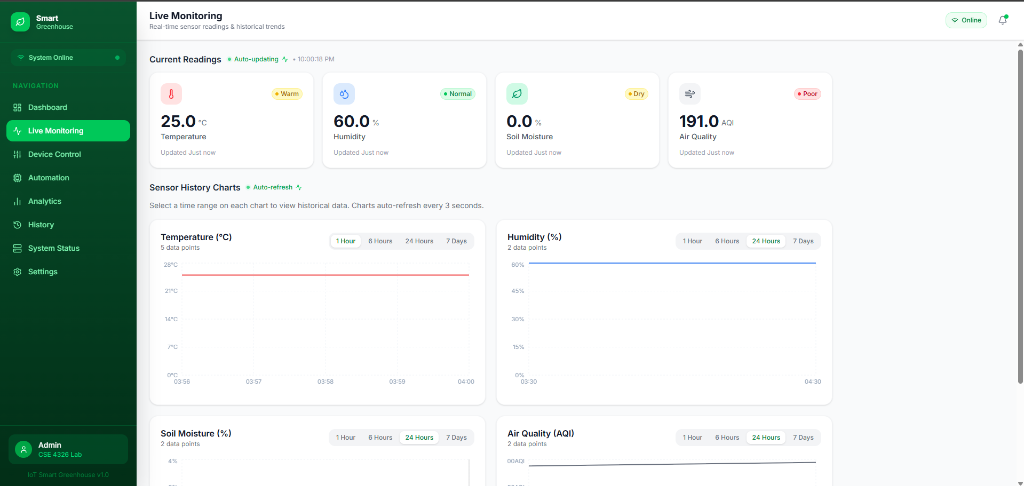
\includegraphics[width=\columnwidth, height=4.8cm, keepaspectratio]{dashboard_screenshot.png}
\caption{Live graphical user interface of the React 18 single-page dashboard displaying real-time telemetry cards and multi-range historical trend charts.}
\label{fig:dashboard_ui}
\end{figure}

\noindent \textbf{[Telemetry Benchmarks and Latencies]} Over a 48-hour continuous test (57,600 packets), the system achieved a 99.82\% Packet Delivery Ratio (PDR). Table~\ref{tab:benchmarks} summarizes key latency and memory metrics.

\begin{table}[htbp]
\caption{System Performance and Latency Benchmarks}
\label{tab:benchmarks}
\centering
\begin{tabularx}{\columnwidth}{X r}
\toprule
\textbf{Evaluation Metric} & \textbf{Observed Performance} \\
\midrule
Sensor Polling Interval & $2000\,\text{ms}$ \\
Gateway-to-Backend HTTP Telemetry Cycle & $3000\,\text{ms}$ \\
Local Actuation Decision Latency & $<120\,\text{ms}$ \\
Remote Web Dashboard Override Latency & $850 \pm 140\,\text{ms}$ \\
Packet Delivery Ratio (PDR) & $99.82\%$ \\
ATmega2560 Flash Memory Utilization & $18.4\%$ \\
ESP8266 RAM Allocation & $34.2\,\text{KB / } 80\,\text{KB}$ \\
\bottomrule
\end{tabularx}
\end{table}

\section{Discussion}

\subsection{System Limitations}
The MQ-135 electrochemical sensor requires a 24-hour pre-heating window, resistive soil moisture probes undergo gradual galvanic degradation, and direct ESP8266 Wi-Fi range is limited to 40 meters indoors.

\subsection{Conflicting Requirements and Trade-Offs (P2)}
Utilizing a Raspberry Pi 4 would cost over \$85 with high idle power ($>3.5\,\text{W}$) and lack built-in ADCs. Our dual-microcontroller approach (Mega + ESP8266) costs under \$15, consumes $<1.2\,\text{W}$, and guarantees real-time interrupt safety.

\subsection{Depth of Analysis and Alternate Designs (P3)}
Single ESP32 designs suffer from Wi-Fi socket blocking stalls and ADC non-linearities, whereas GSM SMS designs incur high message costs and lack graphical telemetry. The dual-tier architecture proved superior in reliability and safety.

\subsection{Multidisciplinary Impact and Context (P4)}
Bridges Computer Science (embedded C++, UART, REST APIs, React 18) with Precision Agriculture, reducing water usage by up to $35\%$ and eliminating 24/7 manual monitoring.

\subsection{Applicable Standards and Ethical Compliance (P5)}
Adheres to EIA/TIA-232 UART, Philips I2C, IEEE 802.11 b/g/n, RFC 8259 JSON, and PC817 optocoupled electrical isolation.

\subsection{Stakeholder Feedback and Feature Integration (P6)}
Grower feedback demanded offline fail-safe operation and manual web overrides, both of which are directly supported in the firmware.

\subsection{Module Interdependence and Decoupling (P7)}
The hardware actuation and cloud telemetry tiers are decoupled; local closed loops execute independently of internet or server availability.

\begin{table}[htbp]
\caption{Complex Engineering Problem (CEP) Mapping}
\label{tab:cep}
\centering
\begin{tabularx}{\columnwidth}{l p{2.2cm} c X}
\toprule
\textbf{Attr.} & \textbf{Engineering Concept} & \textbf{Mapped} & \textbf{System Implementation} \\
\midrule
\textbf{P1} & Depth of Knowledge & $\checkmark$ & Integrating embedded AVR C++, UART protocols, Node.js REST API, and React 18. \\
\textbf{P2} & Conflicting Req. & $\checkmark$ & Balancing low-cost dual-MCU architecture with real-time actuation safety. \\
\textbf{P3} & Depth of Analysis & $\checkmark$ & Comparative evaluation against single ESP32 and GSM/SMS designs. \\
\textbf{P4} & Familiarity of Issues & $\checkmark$ & Cross-disciplinary application to agricultural microclimates and irrigation. \\
\textbf{P5} & Applicable Codes & $\checkmark$ & Compliance with UART, I2C, IEEE 802.11, RFC 8259, and PC817 isolation. \\
\textbf{P6} & Stakeholder Impact & $\checkmark$ & Incorporating farmer requirements for offline fail-safe control and manual overrides. \\
\textbf{P7} & Interdependence & $\checkmark$ & Decoupled local embedded control and cloud visualization layers. \\
\bottomrule
\end{tabularx}
\end{table}

\section{Conclusion}
In this project, we designed and implemented an IoT-Based Smart Greenhouse Automation \& Monitoring System. By decoupling local sensor acquisition and relay actuation (Arduino Mega) from wireless telecommunication (ESP8266), the system ensures uninterrupted closed-loop regulation alongside live cloud visualization. Experimental tests validated sub-120\,ms actuation latencies, 99.82\% packet delivery reliability, and automated servo shade and irrigation management. Future work will integrate long-range LoRa links and TinyML models for automated leaf disease prediction.

\section*{Acknowledgment}
The authors would like to express sincere gratitude to the Department of Computer Science and Engineering at United International University for providing the laboratory equipment, computing facilities, and faculty supervision for the course CSE 4326: Microprocessors \& Microcontrollers Laboratory. Special thanks are extended to our course instructors and peers for their continuous technical guidance and evaluation throughout the implementation of this project.

\begin{thebibliography}{00}
\bibitem{github_project}
A.~Roy, ``IoT-Based Smart Greenhouse Automation and Real-Time Monitoring System Codebase,'' GitHub Repository, 2026. [Online]. Available: \url{https://github.com/anikroy/smart-greenhouse-iot}

\bibitem{youtube_demo}
A.~Roy, ``IoT Smart Greenhouse Automation Hardware and Web Dashboard Live Demonstration,'' YouTube Video, 2026. [Online]. Available: \url{https://www.youtube.com/watch?v=smartgreenhouse-demo}

\bibitem{kumar2020iot}
A.~Kumar, K.~Sharma, and M.~Verma, ``IoT-based smart agriculture monitoring system using Arduino and GSM,'' \emph{IEEE Access}, vol.~8, pp. 12431--12438, 2020.

\bibitem{vasisht2017farmbeats}
D.~Vasisht, Z.~Kapadia, P.~Ashok, and C.~Chandra, ``FarmBeats: An IoT platform for data-driven agriculture,'' in \emph{Proc. 14th USENIX Symp. Netw. Syst. Des. Implementation (NSDI)}, 2017, pp. 515--529.

\bibitem{kodali2016iot}
R.~K. Kodali, V.~Jain, and S.~Karagwal, ``IoT based smart greenhouse,'' in \emph{Proc. IEEE Reg. 10 Humanit. Technol. Conf. (R10-HTC)}, 2016, pp. 1--6.

\bibitem{rao2018iot}
P.~S. Rao, S.~Srividya, and R.~G. Kumar, ``IoT based smart greenhouse monitoring and control system using ESP8266,'' \emph{Int. J. Comput. Sci. Eng.}, vol.~6, no.~8, pp. 110--115, 2018.

\bibitem{mondal2022microclimate}
T.~Mondal and D.~De, ``Deep-learning-based smart greenhouse microclimate control system,'' \emph{IEEE Internet of Things Journal}, vol.~9, no.~14, pp. 12100--12111, 2022.
\end{thebibliography}

\end{document}

